\section{Configuración de la espada}

Ya se ha explicado en otras secciones por separado, pero me gustaría repetirlo todo de nuevo en una sola sección para más claridad.

\bigskip

La espada tiene dos restricciones, que dividiré en subsecciones distintas a continuación:

\subsection{Position Constraint}

Para que la espada se quede pegada a las manos y a la plataforma, es necesario usar el \textit{Position Constraint} cuyos objetivos sean ambas manos y un \textit{dummy} que hay en la plataforma.

\bigskip

Para realizar el cambio de un objeto a otro, es necesario cambiar sus pesos mediante \textit{keyframes}. Por tanto, los instantes más importantes son: 

\begin{itemize}
    \item \textbf{Instante 20: }El peso de la restricción se encuentra en la mano izquierda del todo.
    \item \textbf{Instante 27: }Ahora el peso de la restricción se encuentra del todo en la otra mano.
    \item \textbf{Instante 65: }El peso se sigue manteniendo en la mano derecha.
    \item \textbf{Instante 70: }Ahora el peso se encuentra en el \textit{dummy} de la plataforma.
\end{itemize}

\bigskip

Las curvas de animación son:

\begin{figure}[H]
    \centering
    % curvas
    \begin{subfigure}[t]{0.27\textwidth}
        \centering
        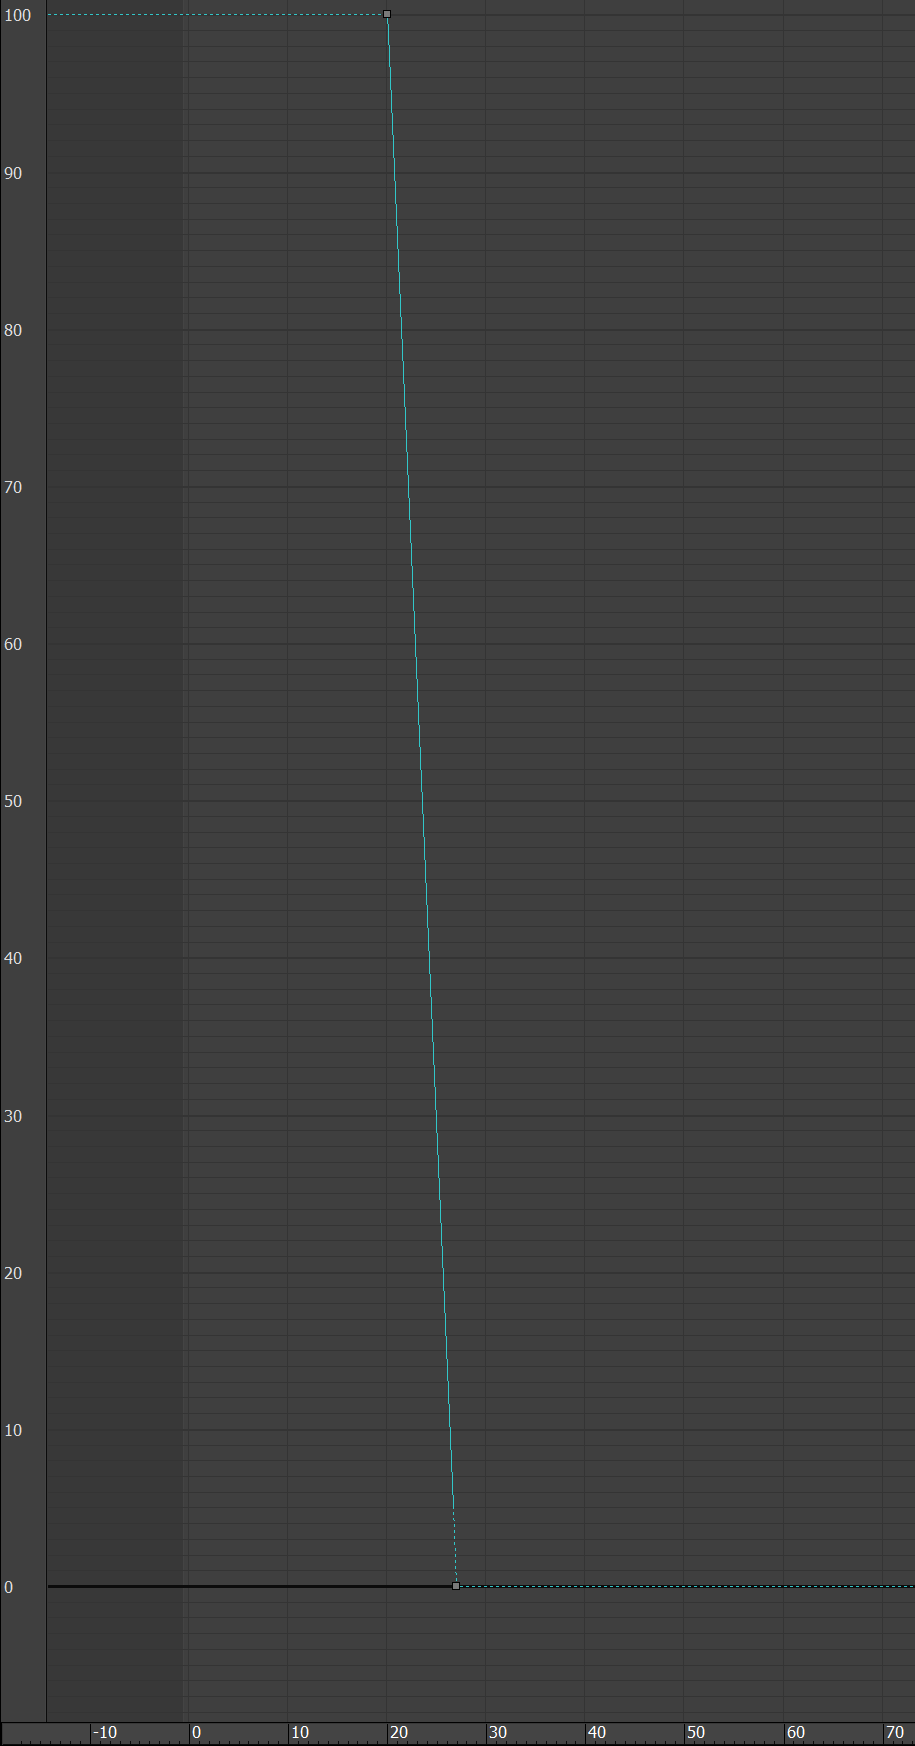
\includegraphics[width=\textwidth]{imagenes/espada/peso0.png}
        \caption{Curva que representa el peso de la mano izquierda con respecto al tiempo.}
     \end{subfigure}
    \hfill
     \begin{subfigure}[t]{0.27\textwidth}
        \centering
        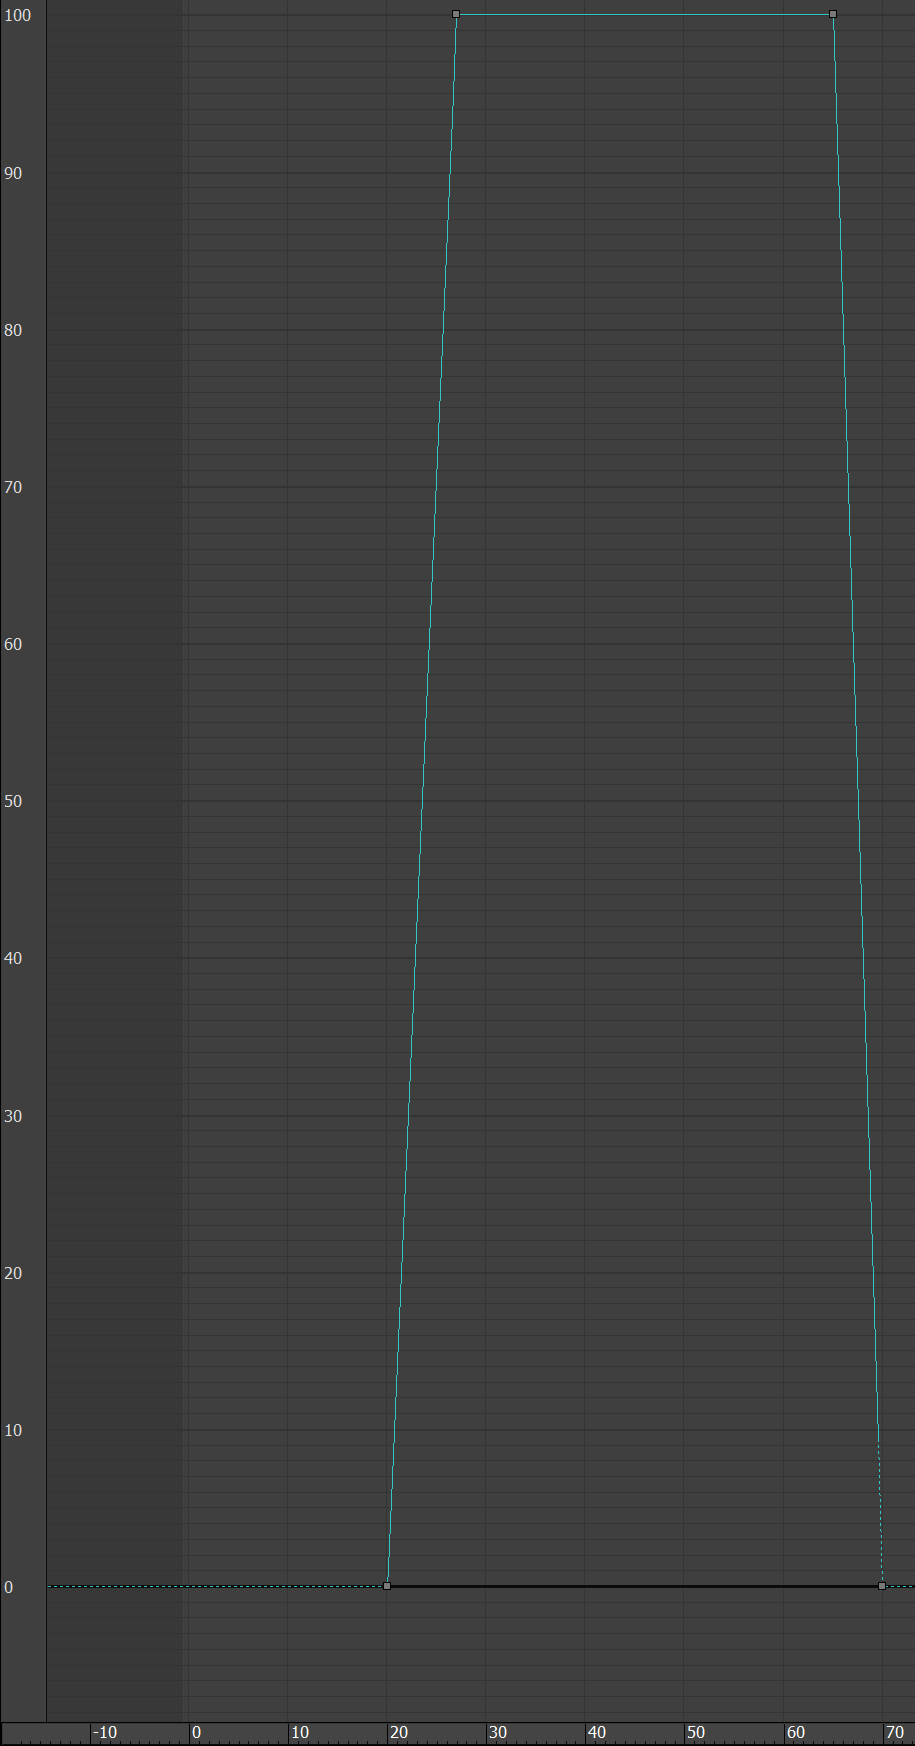
\includegraphics[width=\textwidth]{imagenes/espada/peso1.png}
        \caption{Curva que representa el peso de la mano derecha con respecto al tiempo.}
     \end{subfigure}
    \hfill
     \begin{subfigure}[t]{0.27\textwidth}
        \centering
        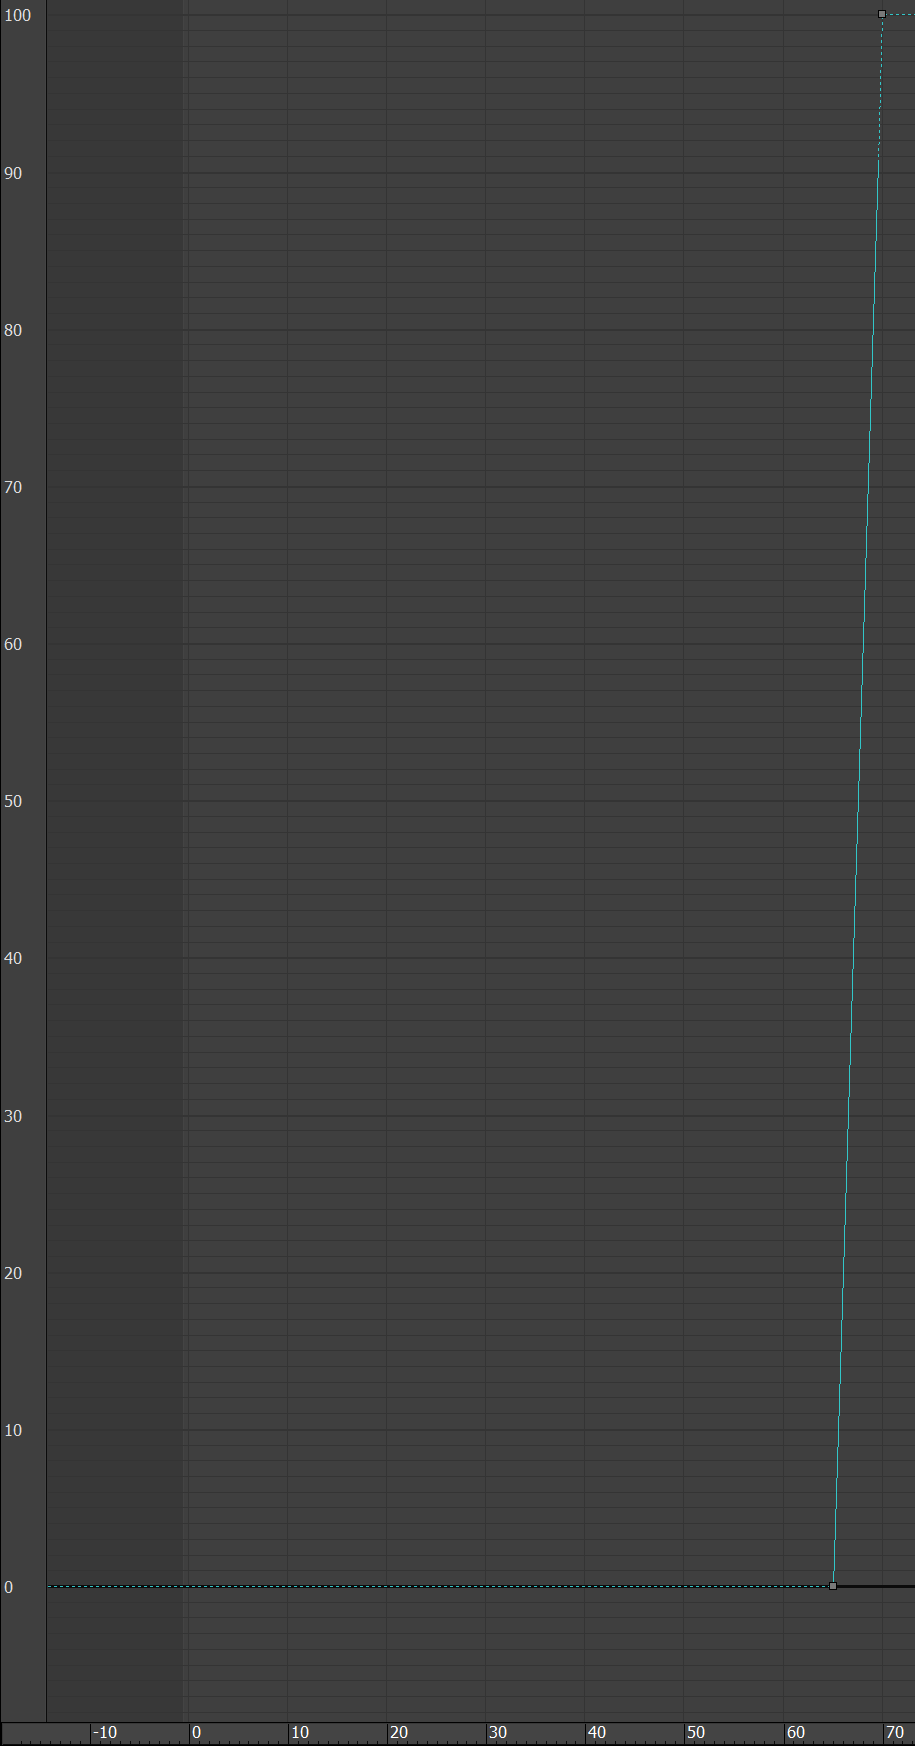
\includegraphics[width=\textwidth]{imagenes/espada/peso2.png}
        \caption{Curva que representa el peso de la plataforma con respecto al tiempo.}
     \end{subfigure}
     \caption{Curvas de los pesos del \textit{Position Constraint}.}
 \end{figure}

Como dije en la sección de las manos, he usado para el cambio de manos una curva de aceleración y al final lineal, para simular el lanzamiento de la espada de una mano a otra. En cuanto al cambio de la plataforma, al no tener animación el cambio de pesos, he decidido hacerlo también para ser consistente.


\bigskip

El resultado final es que la espada pasa de una mano a otra, después la mano de la derecha deja la espada en la plataforma y finalmente la grúa se mueve con la espada encima.


\subsection{LookAt Constraint}

Una vez que la espada ha subido en la plataforma, es necesario hacer que siga el recorrido del coche. Para ello se debe usar un \textit{LookAt Constraint} en el eje Z, que permite fijarse en el objeto que tenga como objetivo. 

\bigskip

No obstante, si solo se elige como objetivo el coche, la espada quedará torcida desde un primer momento, ya que va a estar mirándolo. Una forma de solucionarlo es usando un \textit{Dummy} con una restricción \textit{Link} en las manos y la plataforma, para que siga siempre encima de la espada. Además, he limitado el movimiento de esta restricción a solo la translación en los 3 ejes.

\bigskip

Como dije en el apartado del coche, esto se puede hacer yendo a: \textit{Hierarchy} $\rightarrow$ \textit{Link Info}.

\begin{figure}[H]
    \centering
   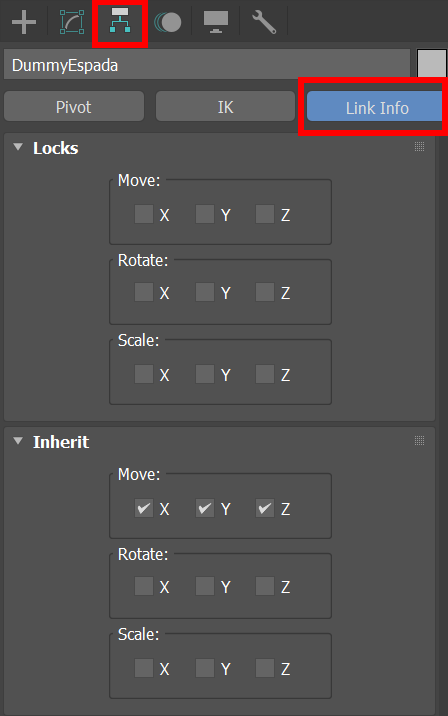
\includegraphics[width=0.35\textwidth]{imagenes/espada/dummyTopHierarchy.png}
   \caption{Menú para bloquear canales.}
\end{figure}

Poniendo como objetivo en el \textit{LookAt Constraint} este \textit{dummy}, ya se ha solucionado el problema, pero hay que cambiar el peso cuando la espada se encuentre arriba para que mire al coche.

\bigskip

Por tanto, los \textit{keyframes} son:

\begin{itemize}
    \item \textbf{Instante 125: }El peso de la restricción está completamente en el \textit{dummy} superior.
    \item \textbf{Instante 150: }El peso de la restricción está completamente en el \textit{dummy} del coche para que lo siga en su trayecto.
\end{itemize}

\bigskip

La curva de animación es las siguientes:

\begin{figure}[H]
    \centering
   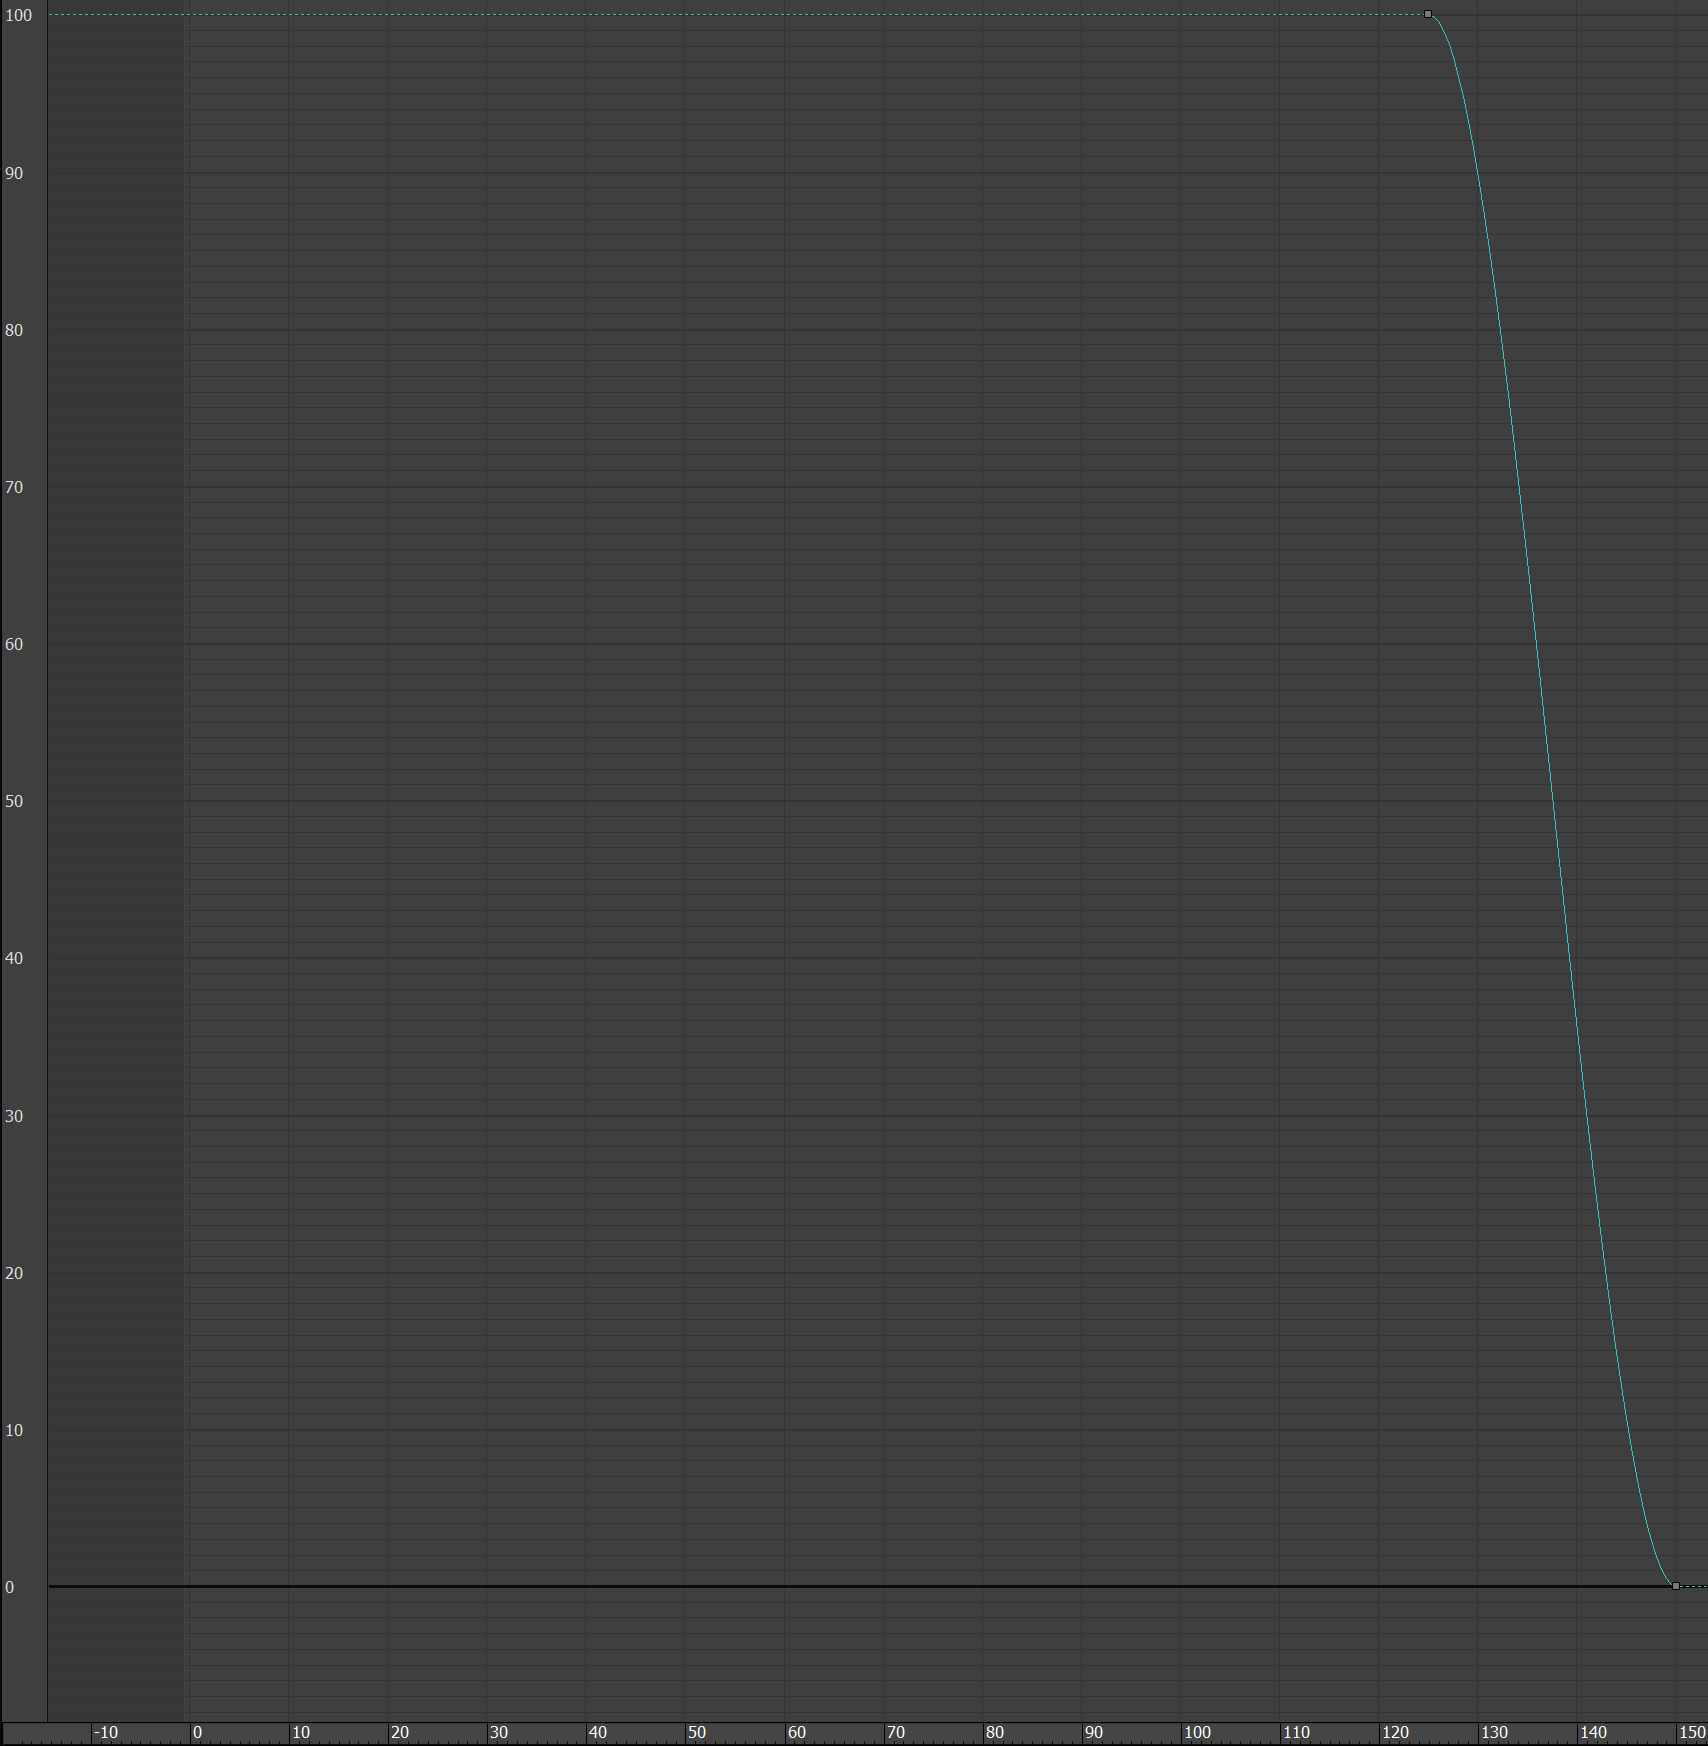
\includegraphics[width=0.6\textwidth]{imagenes/espada/lookat0.png}
   \caption{Curva usada para realizar el cambio de pesos en la restricción en el objetivo del \textit{dummy}.}
\end{figure}

\begin{figure}[H]
    \centering
   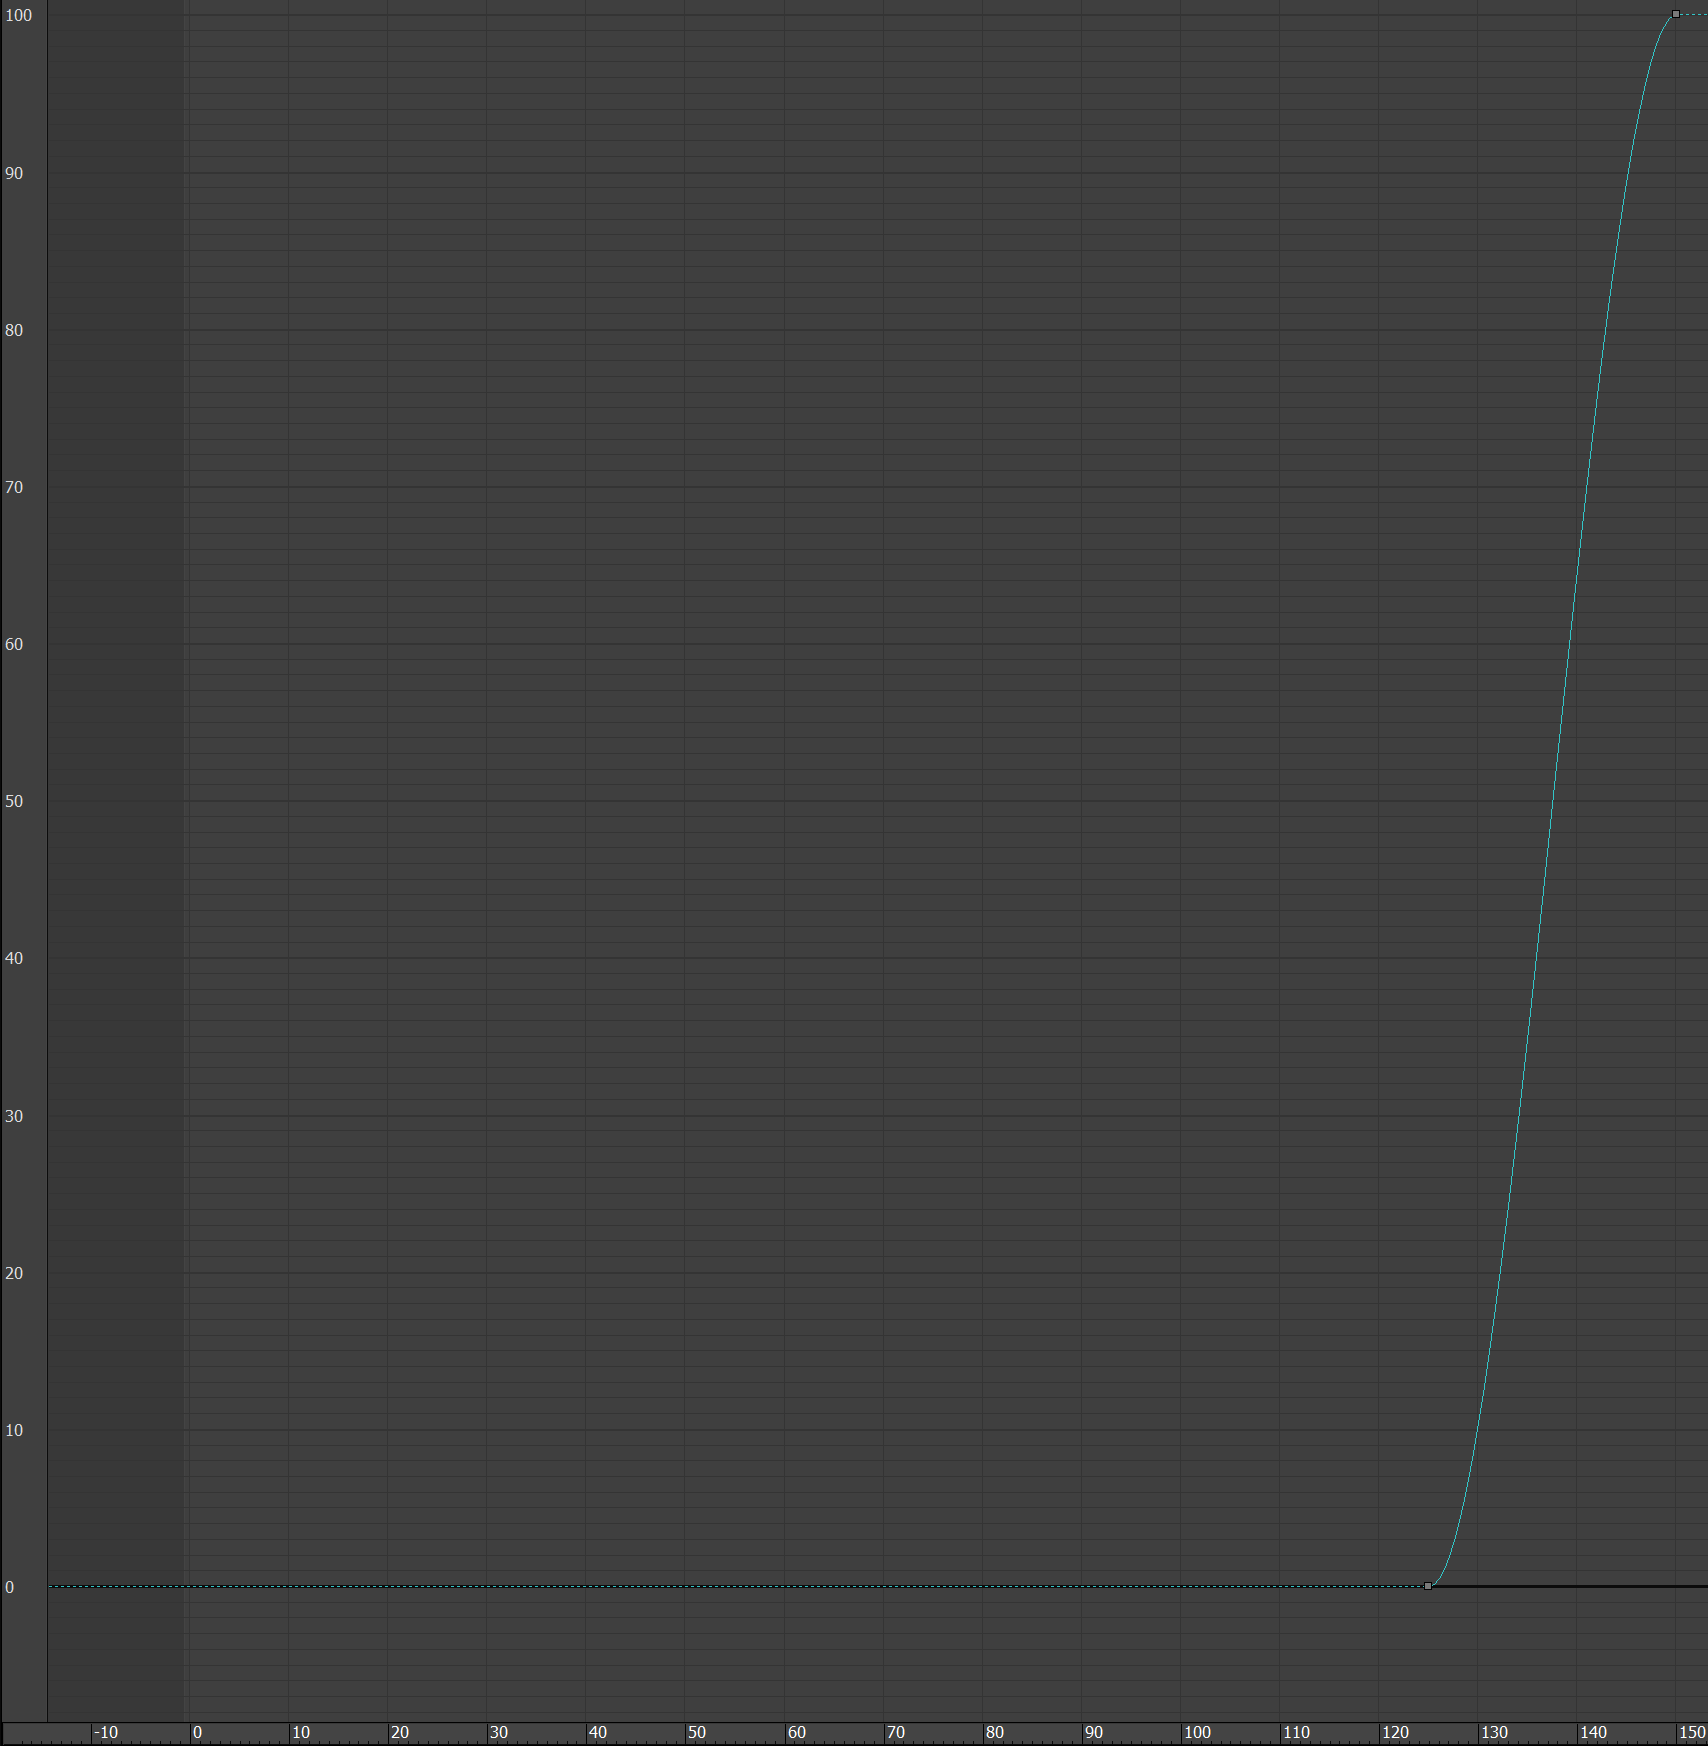
\includegraphics[width=0.6\textwidth]{imagenes/espada/lookat1.png}
   \caption{Curva usada para realizar el cambio de pesos en la restricción en el objetivo del \textit{dummy} del coche.}
\end{figure}

Como se puede observar, he usado la forma por defecto, ya que es la que me ha resultado más suave y realista.
